\documentclass[11pt, a4paper]{article}
\usepackage[utf8]{inputenc}
\usepackage[english]{babel}
\usepackage{amsmath}
\usepackage{amsthm}
\usepackage{amsfonts}
\usepackage{amssymb}
\usepackage{graphicx}
\usepackage{tikz}
\usepackage{listings}
\usepackage[justification=centering]{caption}
\usetikzlibrary{arrows, automata, graphs, shapes, petri, decorations.pathmorphing}
\parindent = 0pt

% define environments
\theoremstyle{definition}
\newtheorem{definition}{Definition}

\theoremstyle{plain}
\newtheorem{theorem}[definition]{Theorem}
\newtheorem{lemma}[definition]{Lemma}

\renewcommand{\labelenumi}{(\roman{enumi})}
\renewcommand{\labelenumi}{(\roman{enumi})}

\author{Niklas Rieken}
\title{Myhill-Nerode-Äquivalent und Pumping-Argumente}


\begin{document}
\maketitle

In diesem Dokument geht es um die Myhill-Nerode-Äquivalenz und ihre Anwendungen für reguläre Sprachen. Sie liefern vorallem ein notwendiges und hinreichendes Bedingung dafür ob eine Sprache regulär ist oder nicht. Der in der Vorlesung (zu Unrecht, meiner Meinung nach) am meisten beworbene Weg um zu zeigen, dass eine Sprache nicht regulär ist, ist die Anwendung des Pumping-Lemma, was für viele FoSAP-Hörer das Schreckgespenst der Vorlesung ist, obwohl das dahinter stehende Argument recht einfach ist. Wir zeigen hier einen ähnliches Argument: Es ist nicht genau das Pumping-Lemma. Stattdessen beweisen wir etwas direkter, dass für eine nicht-reguläre Sprache kein endlicher Automat existieren kann.

\section*{Myhill-Nerode-Äquivalenz}
Bisher sind reguläre Sprachen durch Formalismen wie reguläre Ausdrücke und endliche Automaten charakterisiert worden. Nun soll eine Eigenschaft gefunden werden, die reguläre Sprachen auf einer stark mathematisch-struk\-tur\-ellen Ebene charakterisiert, d.h. mit Aussagen, die sich auf die Struktur
\[
	(\Sigma^\ast, \cdot, \varepsilon)
\]
beziehen. Diese Struktur bezeichnet man auch als \textit{Wortmonoid}.

\subsection*{Grundlegende Überlegungen}
Bevor wir zur eigentlichen Definition der Myhill-Nerode-Äquivalenz kommen, wiederholen wir ein paar Definitionen:
\begin{definition}
	Eine \textbf{Äquivalenzrelation} über einer Menge \( A \) ist eine zweistelltige Relation \( \sim \subseteq A \times A \), die 
	\begin{enumerate}
		\item reflexiv (für alle \( x \) gilt \( x \sim x \)),
		\item symmetrisch (wenn \( x \sim y \) dann auch \( y \sim  x \)) und
		\item transitiv (wenn \( x \sim y \) und \( y \sim z \) dann auch \( x \sim z \)) 
	\end{enumerate}
	ist.
\end{definition}

Da die Myhill-Nerode-Relation eigentlich sogar etwas mehr ist, hier noch eine weitere Definition:
\begin{definition}
	Sei \( A \) eine Menge und \( \circ \) eine zweistellige Funktion auf \( A \). Eine Relation \( \sim \subseteq A \times A \) heißt \textbf{rechtsseitige Kongruenz} (bezüglich \( \circ \)), wenn
	\begin{enumerate}
		\item \( \sim \) eine Äquivalenzrelation ist und
		\item \( \circ \) diese Relation respektiert (d.h. für alle \( x \sim y \) und alle \( z \in A \) gilt \( x \circ z \sim y \circ z \)).
	\end{enumerate}
\end{definition}

Die Myhill-Nerode-Äquivalenz ist definiert durch:
\begin{definition}
	Sei \( \Sigma \) ein Alphabet und \( L \subseteq \Sigma^\ast \). Seien \( u, v \in \Sigma^\ast \). \( u \) und \( v \) heißen \textbf{Myhill-Nerode-äquivalent} (\( u \equiv_L v \)) genau dann, wenn für alle \( w \in \Sigma^\ast \) gilt, dass \( uw \in L \) g.d.w. \( vw \in L \).
\end{definition}

Diese Relation ist streng genommen nicht nur eine Äquivalenz sondern auch eine rechtsseitige (!) Kongruenz, deswegen sind auch die Begriffe \textit{Myhill-Nerode-Rechtskongruenz} und -- nicht ganz korrekterweise -- \textit{Myhill-Nerode-Kongruenz} gebräuchlich.

Eine einfacher Folgerung aus der Definition ist
\begin{lemma}\label{kongruenzlemma}
	Sei \( L \subseteq \Sigma^\ast \) eine Sprache. Für alle \( u, v, w \in \Sigma^\ast \) mit \( u \equiv_L v \) gilt
	\[
		uw \equiv_L vw.
	\]
\end{lemma}

Zuletzt der Begriff der Äquivalenzklasse:
\begin{definition}
	Sei \( A \) eine Menge und \( \equiv \subseteq A \times A \) eine Äquivalenzrelation. Eine Menge \( A^\prime \subseteq A \) heißt \textbf{Äquivalenzklasse}, wenn
	\begin{enumerate}
		\item Wenn \( a \in A^\prime \) und \( b \equiv a \), dann ist auch \( b \in A^\prime \),
		\item Für alle \( a, b \in A^\prime \) gilt \( a \equiv b \).
	\end{enumerate}
\end{definition}

Man benennt Äquivalenzklassen auch durch einzelne Repräsentanten, z.B. mit \( [u]_L \) oder \( u/_L \) für die Äquivalenzklasse in der alle Elemente enthalten sind, die zu \( u \) äquivalent sind.
Die Vereinigung aller Äquivalenzklassen zu einer Äquivalenz über einer Menge \( A \) bildet stets eine Partition von \( A \).

\subsection*{Finden der Äquivalenzklassen}
Lemma~\ref{kongruenzlemma} kann dafür verwendet werden um Äquivalenzklassen (der Myhill-Nerode-Äquivalenz \( \equiv_L \)) zu finden. Wir gehen dabei wie folgt vor:\\
Wir starten mit dem leeren Wort \( \varepsilon \) und der zugehörigen Äquivalenzklasse \( [\varepsilon]_L \). Danach wiederholen wir folgende Schritte bis keine neue Äquivalenzklassen mehr gefunden werden:\\
Für jedes Symbol \( a \in \Sigma \) und jede bisher gefundene Äquivalenzklasse \( [u]_L \) betrachte die Äquivalenzklasse \( [ua]_L \). Ist \( [ua]_L = [v]_L \) für eine bereits gefundene Äquivalenzklasse, passiert nichts. Ist dies nicht der Fall, fügen wir \( [ua]_L \) als neue Äquivalenzklasse hinzu.\par
Beachte, dass dieses Verfahren nur für reguläre Sprachen terminiert. Nicht-reguläre Sprachen haben unendlich viele Äquivalenzklassen (s. Satz~\ref{nerode}).\par
Dazu machen wir ein Beispiel. Sei 
\[
	L = \{ w \in \{ a, b \}^\ast \mid w \text{ beginnt mit } b \text{ und nach jedem } a \text{ folgt sofort ein } b \}.
\]
\begin{itemize}
	\item Jedes Wort aus \( \{ a, b \}^\ast \) hat eine Äquivalenzklasse, also auch \( \varepsilon \). Wir bezeichnen diese mit \( [\varepsilon]_L \).
	\item Betrachte nun \( [\varepsilon a]_L = [a]_L \). Es ist \( [a]_L \neq [\varepsilon]_L \) (also \( a \not\equiv_L \varepsilon \)), da \( b \) die Wörter trennt, d.h. \( a \cdot b \notin L \), aber \( \varepsilon \cdot b \in L \). d.h. \( [a]_L \) ist eine neue Äquivalenzklasse.
	\item Betrachte nun \( [\varepsilon b]_L = [b]_L \). Es ist \( [b]_L \neq [\varepsilon]_L \), da \( \varepsilon \) die Wörter trennt, d.h. \( b \cdot \varepsilon \in L \), aber \( \varepsilon \cdot \varepsilon \notin L \). Außerdem \( [b]_L \neq [a]_L \), weil \( \varepsilon \) die Wörter trennt, d.h. \( b \cdot \varepsilon \in L \), aber \( a \cdot \varepsilon \notin L \).
	\item Betrachte nun \( [aa]_L \). Es ist \( [aa]_L = [a]_L \), da es kein trennendes Wort gibt (egal, was man anhängt, man kann nicht mehr in der Sprache landen in beiden Fällen, da das Wort nicht mit \( b \) beginnt).
	\item Betrachte nun \( [ab]_L \). Es ist \( [ab]_L = [a]_L \), da es kein trennendes Wort gibt (egal, was man anhängt, man kann nicht mehr in der Sprache landen in beiden Fällen, da das Wort nicht mit \( b \) beginnt).
	\item Betrachte nun \( [ba]_L \). Es ist \( [ba]_L = [\varepsilon]_L \), da es kein trennendes Wort gibt.
	\item Betrachte nun \( [bb]_L \). Es ist \( [bb]_L = [b]_L \), da es kein trennendes Wort gibt.
	\item Damit sind alle Äquivalenzklassen gefunden: \( [\varepsilon]_L, [a]_L, [b]_L \). Dieser Punkt ist für viele Studenten oft erstmal schwierig zu sehen. Es folgt aber direkt aus der rechtsseitigen Kongruenz bzw. Lemma~\ref{kongruenzlemma}. Egal welches Wort wir betrachten, wir können es einer dieser Äquivalenklassen zuordnen. Betrachte zum Beispiel \( [bab]_L \). Wegen \( ba \equiv_L \varepsilon \) ist \( ba \cdot b \equiv_L \varepsilon \cdot b = b \) und somit \( [bab]_L = [b]_L \). 
\end{itemize}

\subsection*{Wofür ist das nützlich?}
Die Myhill-Nerode-Äquivalenz ist inhaltlich eines der schönsten Sachen in FoSAP, weil sie 1. eine notwendige und hinreichende Bedingung liefert, dass eine Sprache regulär ist und weil sie 2. auch einen direkten Weg zu einem minimalen deterministischen endlichen Automaten liefert.
\begin{theorem}[Satz von Nerode]\label{nerode}
	Eine Sprache ist genau dann regulär, wenn die Anzahl der Myhill-Nerode-Äquivalenzklassen endlich ist.
\end{theorem}
Man schreibt auch \( index(\equiv_L) < \infty \). Die Sprache \( L \) im Beispiel hat \( index(\equiv_L) = 3 < \infty \) und ist somit regulär. Betrachte nun ein Standardbeispiel für eine nicht-reguläre Sprache 
\[
	K = \{ a^n b^n : n \in \mathbb{N} \}.
\]
\( K \) ist nicht regulär. Betrachte die Wörter \( u_i = a^i \) und \( u_j = a^j \) mit \( i \neq j \). Es gilt offensichtlich \( u_i \not\equiv_K u_j \), denn das Wort \( b^i \) trennt die Wörter, weil \( u_i b^i = a^i b^i \in K \), aber \( u_j b^i = a^j b^i \notin K \). Da es unendlich viele \( i, j \in \mathbb{N} \) mit \( i \neq j \) gibt, gibt es auch unendlich viele Äquivalenzklassen. Also ist \( K \) nach dem Satz von Nerode nicht regulär.

\begin{theorem}
	Der minimale DFA zu einer reguläre Sprache \( L \) ist isomorph zum Myhill-Nerode-DFA:
	\[
		\mathcal{A}_L = (\Sigma^\ast/_L, \Sigma, \delta, [\varepsilon]_L, \{[u]_L : u \in L \}),
	\]
	mit \( \delta([u]_L, a) = [ua]_L \).
\end{theorem}
Für die Sprache \( L \) erhalten wir also den DFA in Abbildung~\ref{fig:mindfa}.
\begin{figure}
	\centering
	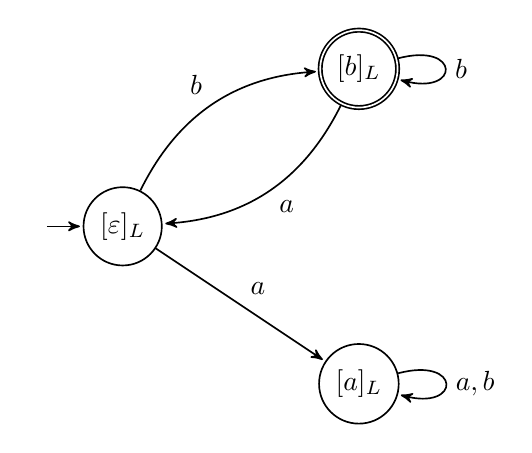
\begin{tikzpicture}[->, >=stealth', shorten >=1pt, auto, semithick]
		\node[state, initial, initial text=] (0) at (0, 0) {$[\varepsilon]_L$};
		\node[state] (1) at (3, -2) {$[a]_L$};
		\node[state, accepting] (2) at (3, 2) {$[b]_L$};

		\path (0) edge node {$a$} (1)
			(0) edge[bend left] node {$b$} (2)
			(1) edge[loop right] node {$a, b$} (1)
			(2) edge[bend left] node {$a$} (0)
			(2) edge[loop right] node {$b$} (2);
	\end{tikzpicture}
	\caption{Minimaler DFA für die Sprache \( L \).}
	\label{fig:mindfa}
\end{figure}


\section*{Pumping-Argumente}
Dies ist ein Thema mit der viele Studenten in der Regel Probleme haben, da das Pumping-Lemma etwas sperrig ist und nicht sehr natürlich wirkt. Zur Erinnerung aber trotzdem nochmal:\par
Sei \( L \) eine reguläre Sprache. Dann existiert ein \( n \in \mathbb{N}_+ \), sodass für alle \( w \in L \) mit \( \left| w \right| \geq n \) eine Zerlegung \( w = xyz \) existiert für die gilt:
\begin{enumerate}
	\item \( \left| xy \right| \leq n \),
	\item \( y \neq \varepsilon \),
	\item \( xy^i z \in L \) für alle \( i \in \mathbb{N} \).
\end{enumerate}
Wir betrachten jetzt die Sprache 
\[
	L = \{ uav \,\vert\, u, v \in \{ a, b \}^\ast \text{ mit } \left| u \right| = \left| v \right| \} 
\]
Der herkömmliche Weg, der auch in der Vorlesung vorgestellt wurde ist nun genau dieses Lemma benutzen und die Annahme, dass \( L \) regulär ist zu einem Widerspruch zu führen. Das ist aber genau das womit viele Schwierigkeiten haben, deswegen versuche ich das hier etwas anschaulicher:\par
Angenommen \( L \) ist regulär, dann gibt es einen endlichen Automaten \( \mathcal{A} = (Q, \Sigma, \Delta, q_0, F) \), der \( L \) erkennt. Angenommen \( \mathcal{A} \) habe \( n \) Zustände. Wir betrachten das Wort \( w = b^n a b^n \). Das Wort ist in der Sprache und hat die Länge \( 2n+1 > n \). Nach Lesen des Präfix \( b^n \) muss also spätestens eine Zustandswiederholung im akzeptierenden Lauf von \( \mathcal{A} \) auf \( w \) aufgetreten sein (\textit{pigeonhole principle, Schubfachprinzip}), d.h. vor dem Lesen vom \( a \). Wir nehmen an, der Zustand, der sich wiederholt trat nach Lesen des \(i\)-ten und \(j\)-ten (oBdA \( j > i \)) \( b \) auf (s. Abbildung~\ref{fig:pl}). Wir betrachten also den Lauf
\[
	r = (q_0, b,  q_1, \ldots, b, q_i, b, \ldots, q_j, b, q_{j+1}, \ldots, b, q_n, a, q_{n+1}, b, \ldots, b, q_{2n+1}),
\]
mit \( q_{2n+1} \in F \) wobei \( q_i = q_j \). Sei \( j-i = k > 0 \). Der Lauf 
\[
	r = (q_0, b, \ldots, q_i, b, q_{j+1}, \ldots, b, q_{2n+1})
\]
ist also ebenfalls möglich und auch akzeptierend mit dem Wort \( w^\prime = b^{n-k}ab^n \), aber \( w^\prime \notin L \), also erkennt \( \mathcal{A} \) nicht die Sprache mit \( n \) Zuständen. Da \( n \) beliebig war gibt es also keinen endlichen Automaten, der \( L \) akzeptiert. Somit folgt, dass \( L \) nicht regulär ist.\par
Man sieht vielleicht, dass in dieser Lösung die Wörter und Zahlen aus dem Pumping Lemma wieder auftauchen, was natürlich kein Zufall ist (\( n \), Das Präfix \( b^j \) entspricht \( xy \), das Infix \( b^k \) mit \( k > 0 \) entspricht \( y \) und das Weglassen von \( b^k \) in \( w^\prime \) entspricht der Betrachtung von \( xz \) in \textit{iii)}).
\begin{figure}
	\centering
	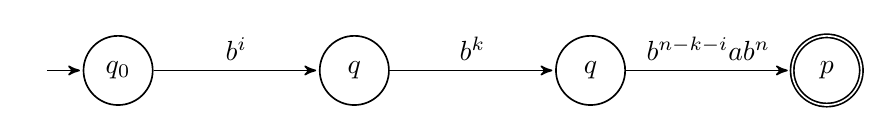
\begin{tikzpicture}[->, >=stealth', shorten >=1pt, auto, semithick]
		\node[state, initial, initial text=] (0) at (0, 0) {$q_0$};
		\node[state] (i) at (3, 0) {$q$};
		\node[state] (j) at (6, 0) {$q$};
		\node[state, accepting] (p) at (9, 0) {$p$};
		
		\path (0) edge node {$b^i$} (i)
			(i) edge node {$b^k$} (j)
			(j) edge node {$b^{n-k-i}ab^n$} (p);
	\end{tikzpicture}
	\caption{Zustandswiederholung in \( q \). Es gibt also einen Lauf von \( q_0 \) nach \( q \) und einen Lauf von \( q \) nach \( p \). Den Zwischenlauf von \( q \) nach \( q \) kann man also weglassen (oder auch beliebig oft wiederholen).}
	\label{fig:pl}
\end{figure}

\end{document}